% Architectural support for building scalable, resilient and high-performance NFV system
\section{Evaluation}
\label{sec:evaluation}

%We present an initial micro-benchmark of Netstar framework. In this micro-benchmark, we generate a large number of UDP flows (100000) running at 10Gbps/s (14.4 Mpps/s). These UDP flows are send to an NF running Netstar framework. For each received packet, the NF will use the flow-5-tuple as the key to perform several database queries. The queries consist of interleaved read/write request. The write request writes to the database a 24-bytes long value while the read request read the 24-bytes long value back. The NF runs on a server with 10 physical cores. We vary the number of the queries per packet to see the throughput performance achieved by Netstar. The result is presented in figure \ref{fig:benchmark}.

%We can see from figure \ref{fig:benchmark} that at the most extreme case, the NF can process 2M packets per second while querying the database 14M times.

%\begin{figure}[!t]
%  \centering
%  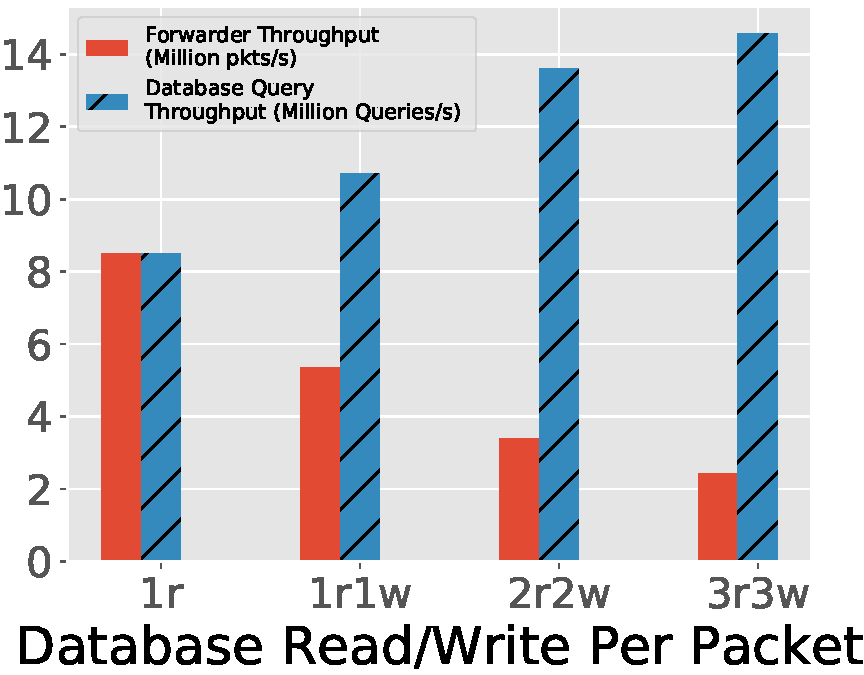
\includegraphics[width=\columnwidth]{figure/micro_latency.pdf}
%  %\vspace{-2mm}
%  \caption{Microbenchmark.}
%  \label{fig:benchmark}
%  %\vspace{-6mm}
%\end{figure}

\subsection{Micro Benchmark}

In this section, we show micro benchmark of NetStar. We are showing four benchmarks here.

First as shown in Fig.~\ref{benchmark1}, micro benchmark of packet forwarding rate under different packet size, including the comparison with a pure DPDK based implementation, together with our optimization result.

\begin{figure}[!t]
  \centering
  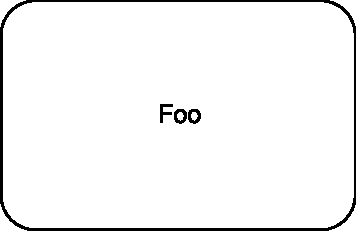
\includegraphics[width=0.5\columnwidth]{figure/foo.pdf}
  \caption{Packet forwarding throughput.}
  \label{benchmark1}
\end{figure}

Second as shown in Fig.~\ref{benchmark2}, the latency CDF of 64 bytes between NetStar and a DPDK based implementation.

\begin{figure}[!t]
  \centering
  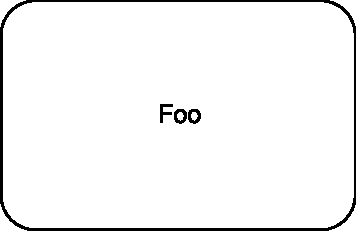
\includegraphics[width=0.5\columnwidth]{figure/foo.pdf}

  \caption{Packet forwarding latency cdf.}
  \label{benchmark2}

\end{figure}

Third as shown in Fig.~\ref{benchmark3}, micro benchmark of asynchronous query. Using mica server read-write as example.

\begin{figure}[!t]
  \centering
  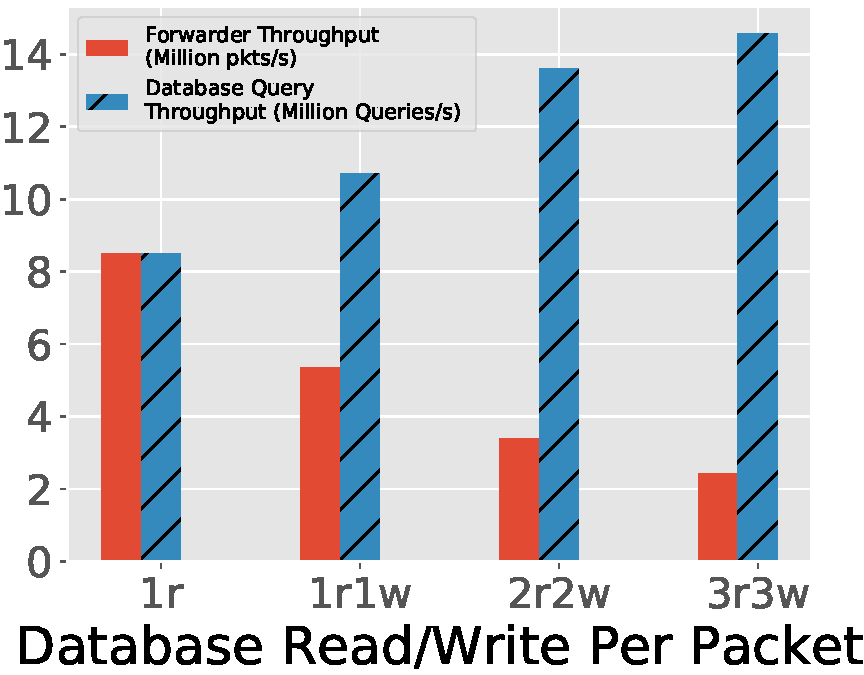
\includegraphics[width=0.5\columnwidth]{figure/micro_latency.pdf}

  \caption{Packet forwarding throughput while query database.}
  \label{benchmark3}

\end{figure}

Fourth as shown in Fig.~\ref{benchmak4}, the latency CDF of 64 bytes packets when there is 1-read and 3-read-3-write.

\begin{figure}[!t]
  \centering
  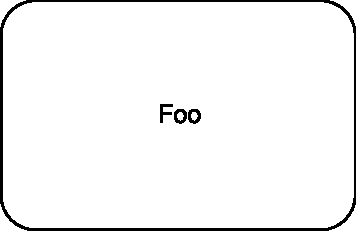
\includegraphics[width=0.5\columnwidth]{figure/foo.pdf}

  \caption{Packet forwarding latecy cdf while querying database.}
  \label{benchmark4}

\end{figure}

\subsection{Evaluation of NFs from StatelessNF Paper}

\begin{table}[]
\centering
\caption{My caption}
\label{my-label}
\begin{tabular}{|l|l|l|l|l|}
\hline
NF       & \begin{tabular}[c]{@{}l@{}}future/promise \\ total\end{tabular} & \begin{tabular}[c]{@{}l@{}}callback\\ total\end{tabular} & \begin{tabular}[c]{@{}l@{}}future/promise\\ error handling\end{tabular} & \begin{tabular}[c]{@{}l@{}}callback\\ error handling\end{tabular} \\ \hline
LB       & 541                                                             & 603                                                      & 8                                                                       & 16                                                                \\ \hline
Firewall & 531                                                             & 592                                                      & 8                                                                       & 8                                                                 \\ \hline
NAT      & 576                                                             & 637                                                      & 8                                                                       & 20                                                                \\ \hline
IPS      & 657                                                             & 730                                                      & 8                                                                       & 8                                                                 \\ \hline
\end{tabular}
\end{table}

First as shown in Fig.~\ref{snf1}, forwarding throughput of NFs, together with a callback-based implementation.

\begin{figure}[!t]
  \centering
  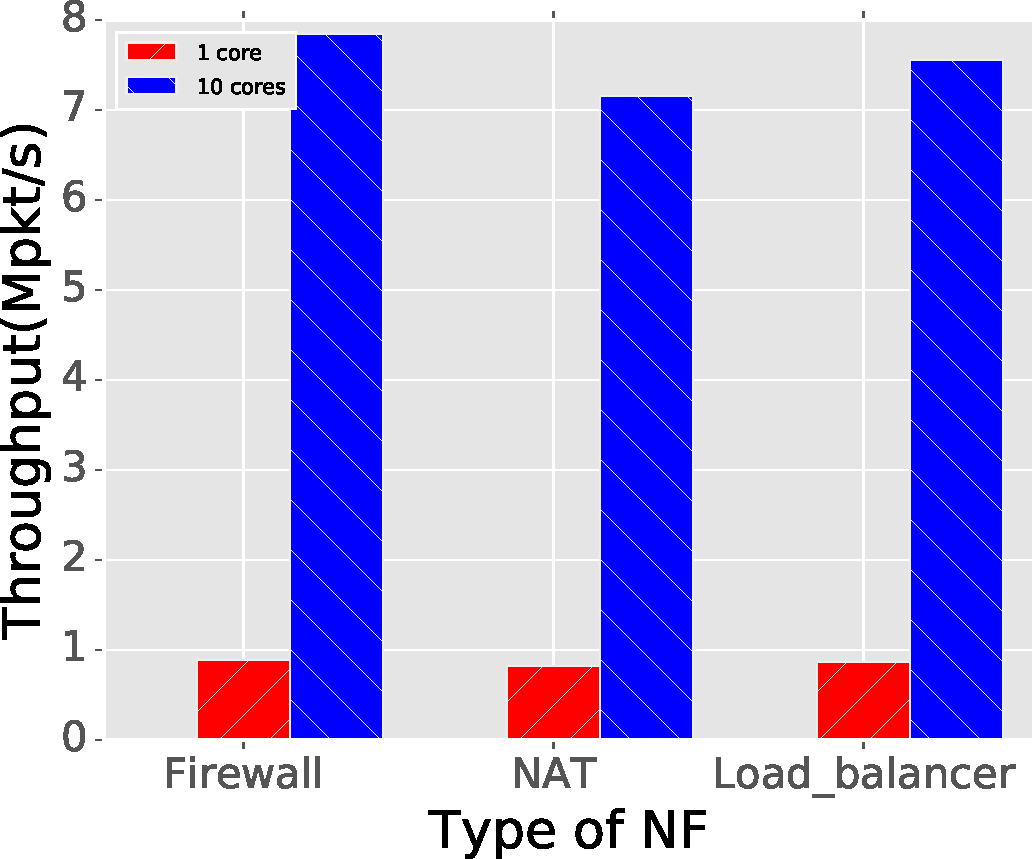
\includegraphics[width=0.5\columnwidth]{figure/Throughput.pdf}
  %\vspace{-2mm}
  \caption{Packet forwarding throughput of NFs according to StatelessNF paper.}
  \label{snf1}
  %\vspace{-6mm}
\end{figure}

Second as shown in Fig.~\ref{snf2}, packet processing latency cdf for 64 bytes packets for both NFs implemented using NetStar and NFs implemented using callback.

\begin{figure}[!t]
  \centering
  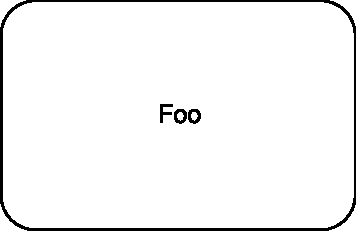
\includegraphics[width=0.5\columnwidth]{figure/foo.pdf}
  %\vspace{-2mm}
  \caption{Packet forwarding latency cdf comparison among NFs implemented using NetStar and NFs implemented using callback.}
  \label{snf2}
  %\vspace{-6mm}
\end{figure}

Third, a table comparing the LoC for implementing the core logic among NFs implemented using NetStar and callback-based implementation.

\subsection{Evaluation of HTTP Reverse Proxy}

First as shown in Fig.~\ref{http1}, HTTP proxy throughput comparison between NetStar, Tiny proxy and HAProxy.

\begin{figure}[!t]
  \centering
  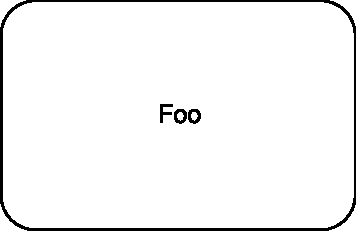
\includegraphics[width=0.5\columnwidth]{figure/foo.pdf}
  %\vspace{-2mm}
  \caption{HTTP proxy throughput throughput comparison}
  \label{http1}
  %\vspace{-6mm}
\end{figure}

Second, comparing the main LoC for implementation in a table.

\subsection{Evaluation of IDS}

First as shown in Fig.~\ref{ids1}, throughput when detecting HTTP traffic containing small request, as well throughput when detecting HTTP traffic containing large request. With a comparison to an IDS implementation based on mOS.

\begin{figure}[!t]
  \centering
  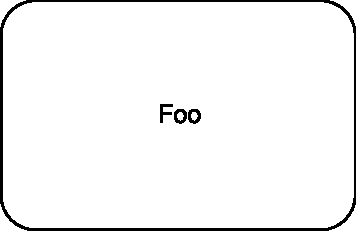
\includegraphics[width=0.5\columnwidth]{figure/foo.pdf}
  %\vspace{-2mm}
  \caption{HTTP traffic throughput IDS comparison}
  \label{ids1}
  %\vspace{-6mm}
\end{figure}

Second as shown in Fig.~\ref{ids2}, file download completion time, with a comparison against mOS. The size of the file is varied.

\begin{figure}[!t]
  \centering
  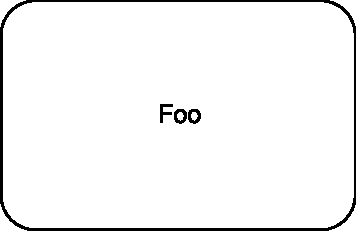
\includegraphics[width=0.5\columnwidth]{figure/foo.pdf}
  %\vspace{-2mm}
  \caption{File download completion time IDS comparison.}
  \label{ids2}
  %\vspace{-6mm}
\end{figure}


Third as shown in Fig.~\ref{ids3}, real-world trace test, and comparison among against IDS.

\begin{figure}[!t]
  \centering
  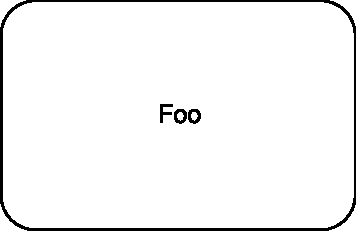
\includegraphics[width=0.5\columnwidth]{figure/foo.pdf}
  %\vspace{-2mm}
  \caption{Real-world trace comparison.}
  \label{ids3}
  %\vspace{-6mm}
\end{figure}

Fourth, a table comparing the implementation LoC.

\subsection{Evaluation of DNS-based Load-balancer}

First as shown in Fig.~\ref{dns1}, throughput comparison of NetStar against an implementation based on callback.

\begin{figure}[!t]
  \centering
  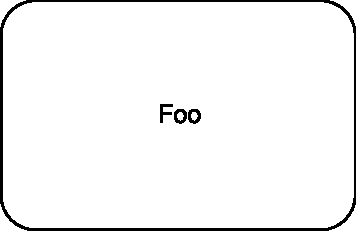
\includegraphics[width=0.5\columnwidth]{figure/foo.pdf}
  %\vspace{-2mm}
  \caption{Throughput comparison between DNS load-balancer implemented using NetStar against callback.}
  \label{dns1}
  %\vspace{-6mm}
\end{figure}

Second, a table compare implementation LoC.
